% Chapter 5

\chapter{Evaluation} % Main chapter title

\label{Evaluation} % For referencing the chapter elsewhere, use \ref{Chapter1} 
%----------------------------------------------------------------------------------------
This chapter will present the evaluation and results of the goals that were set in Chapter \ref{Goals}.\\
At first, approaches will be explained to evaluate the goals and related work will be presented. Following that, the methods will be proposed containing the preprocessing steps and the selection of the training and validation sets with respect to the different approaches. In the last step, results will be presented and discussed.


%----------------------------------------------------------------------------------------
\section{Approaches} \label{approaches}
In this work there were three approaches used to analyze the influence of object roles in the haptic search experiment. For all of them supervised machine learning was used resulting in three different classification problems: \\
\begin{enumerate}
	\item \textbf{Classifying data into object categories:} a model was build to classify the five stimuli that were used in the experiment. At first the model was trained only on the data of objects when they were targets, and secondly on the data when they were distractors. The performance was measured and compared. The goal was to see if the data would be separable at all and to find a fitting model for it.
	
	\item \textbf{Classifying a single object as either target or distractor:} based on the previous problem, a model was trained separately for each object to classify it's data into a target role or a distractor role. 
	
	\item \textbf{Classifying unseen objects into roles:} in this problem, a model was trained on a single object as either target or distractor and tested on a different unseen object with the same role. The goal was to find out if it is possible to classify roles on an unseen object, which would give insight on the feature correlation between objects.       
\end{enumerate}

Combining the results of all these problems, an answer should be given to the question whether humans explore same objects differently in a haptic search task depending on what the target is. Furthermore, an approach to explain the human efficiency could be made by the results. Instead of classifying all explored objects, they distinguish only between two classes: the target object they searched for and a distractor.      
%----------------------------------------------------------------------------------------
\section{Related Work}
This work combines both object categorization based on their various characteristics and haptic search. Researchers had dealt with the specific task of object classification in previous studies. Since material and functional properties could not be captured because the stimuli used were static and not deformable objects, previous work on shape based classification is perhaps the most related work to the proposed approaches.\\
Schneider et. al. \cite{Schneider} used touch sensors in a manipulation robots fingertips to gain low-resolution intensity images from multiple grasping interactions. They applied a bag-of-words approach and clustering techniques to categorize objects based on haptic feedback. Navarro et. al. presented an approach for haptic recognition and evaluation on multi-fingered robot hands based on extracting key features of tactile and kinesthetic data using clustering \cite{Navarro}. Faldella et. al \cite{Faldella} described an approach to robotic haptic recognition using an unsupervised Kohonen self-organizing feature map for performing a match-to-sample classification of three-dimensional objects. Pezzementi et. al.views tactile sensor data as images and applied PCA techniques to identify principal components of identified features and clusters them as well as build per-class histograms as class characteristics \cite{Pezzementi}. Gorges et. al. \cite{Gorges} additionally included passive joints in the tactile sensor system which could help to acquire more information for shape reconstructionn. They used Self-Organizing Maps for identifying haptic key features and a Bayes Classificator for classifying objects. Bhattacharjee et. al. \cite{Bhattacharjee} demonstrated a tactile sensor array covering a robot's forearm to generate haptic time series data during manipulation tasks. They used the processed and dimensionality reduced data to generate feature vectors and classify them with a k-nearest neighbor algorithm for object recognition.
\\\\
Although it is not dealt with categorization of explicit shape features in the previously defined classification problems, the tactile data acquisition, preprocessing and feature extracting used in these works could also be applied for the mentioned approaches. Especially parts of the data sampling and preprocessing pipeline from Bhattacharjee et. al. \cite{Bhattacharjee} was found to be well applicable on the data recorded for this work.

%----------------------------------------------------------------------------------------
\section{Methods}
In this section the pipeline is presented that was used for the classification problems of the evaluation. At first the preprocessing steps will be explained that will turn the raw data into feature vectors that can be used for training. Figure \ref{pipeline} depicts the complete experimental protocol. In the second part it will be described how the data sets for training and validation were generated.

\subsection{Notation}
A number of notations will be used in this work to describe the data sets that were used in the different evaluations. \\
Let $ \Omega := \{(x_{i},y_{i})\}_{i=1,...,N} $ be the data set of one trial where $ N $ is the number of samples in the time series of this trial and the tuple $ (x_{i},y_{i}) $ denotes the feature vector with the corresponding label at time $ i $. Since every trial had one target object that the participant had to search for while the rest of the objects were distractors, the data set can be decomposed in $ \Omega = \Omega_{T} \cup \Omega_{D} $. Here $ \Omega_{T} $ refers to these $ (x,y) $ where $ y=t $ is label of the target object $ t \in \{1,...,5\} $ . On the other hand $ \Omega_{D} $ contains only the labels of distractor objects $ y \in \{1,...,5\}\setminus t $. A complete set $ \Omega_{A} = \Omega_{1} \cup \hdots \cup \Omega_{M} $ describes the set containing all $ M $ trials of participant $ A $.

\subsection{Preprocessing and Feature Extraction}
%\textcolor{red}{Following text has to be adapted to the new notation!}
%Tactile data was recorded from the glove with a frequency of 150Hz and joint angles at 50Hz. The classification problems were evaluated on both only the tactile data and the merged set with tactile data and joint angles. Therefore a preparation step was to sample the tactile data down to 50Hz with assigning every time value of the joint data series the corresponding tactile data vector. This will result in two time series $ T_{i} = \{x_{t} \mid t \in \{0,..,n\}\} $ and $ M_{i} = \{x_{t} \mid t \in \{0,..,m\}\} $, where $ i \in \{1,..,5\}$ describes the trial for object class $i$ and $ T,M $ refers to tactile only data or the merged set with joint angles. Each value represents a vector $x \in \mathbb{R}^{64}$ for tactile data or $ x \in \mathbb{R}^{64+18} $ for the joined set. Every component in the vector corresponds to a sensor of the 64 tactile cells or the 18 bending sensors.\\
The first step in the pipeline was to apply a z-transformation for each sensor separately with $ x_{j}' = \frac{x_{j}-\bar{x}_{j}}{\sigma_{j}} $, where $ x_{j} $ denotes the j-th component of all samples in the time series vector and $ \bar{x}_{j},\sigma_{j} $ are the mean and standard deviation. Standardizing the data to zero mean and unit variance was necessary since the different tactile cells and bending sensors all have various ranges based on the participant's hand, search strategy and some noise which would significantly influence distance based classifiers.\\
Afterwards a time window was chosen to sample data from the time series at consistent intervals to reduce the amount of redundant data. The time series were recorded with 156Hz and 50Hz, resulting in very close or even similar neighboring data points. With this time window, data points were picked that had a predefined time distance to the previously collected sample. In this work, a sampling rate of 10Hz proved itself reliable.\\
The next step was to extract only relevant samples dependent on the classification problem. Since one time series represents the data of a whole trial, just these data points had to be extracted that belong to specific objects, namely the ones to investigate. This had to be done individually for each approach. Only the data points that included no information at all, e.g. when the hand was in the air or outside of the MHSB, were discarded for all approaches. \\
In the last step, the extracted data was concatenated and a low dimensional representation of the data was computed using a feature extraction method. To find an optimal representation, multiple methods were applied in the first experiment and the one resulting in best performance of the model was chosen. These methods were principal component analysis (PCA) and autoencoder (AE) as well as handcrafted features, i.e. only finger sensors, the sum of the sensors on each finger and the maximum value of the sensors for each finger.

\begin{figure}[h]
	%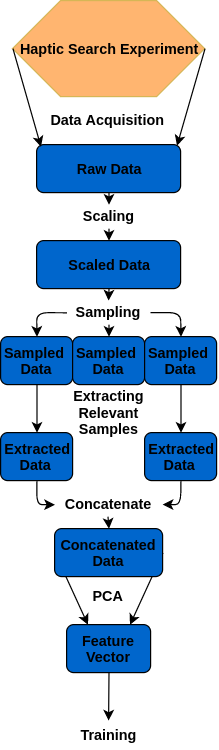
\includegraphics[scale]{Pipeline2}
	\makebox[\textwidth][c]{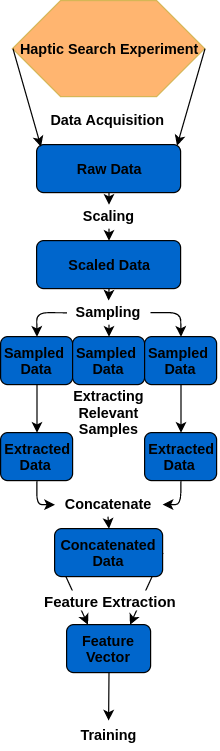
\includegraphics[scale=0.53]{Pipeline2_}}
	\caption{Schematic representation of the complete pipeline}
	\label{pipeline}
\end{figure}

\subsection{Training and Validation Methods}
%To train the feature vector for the classification problems listed in \ref{approaches}, four models were applied on the first task to measure the overall performance for object recognition and to find optimal parameters. It was trained on a k-nearest neighbor model (kNN), a multilayer perceptron (MLP), a support vector machine (SVM) and a random forest classifier. After choosing the winner model, the more specific problems were tackled with it. The results, hyperparameter and model selection is discussed in \ref{results}.\\
For training of the feature vectors and the different extraction methods, a multilayer perceptron (MLP) was applied on the data sets for the classification problems. The first experiment should serve as a baseline to see how well the data can be separated and which feature extraction would prove itself suitable. The MLP consisted of two hidden layers, was using a rectified unit activation function and the lbfgs method as a solver for weight optimization which comes from the family of quasi-Newton methods.\\
\\
A problem that occurred when recording a trial in a single run was that the whole exploration was saved in a sole data frame. Thus the extraction step in the pipeline was necessary to generate data sets suited for the classification experiment.\\
Training was done for each participant separately and scores were averaged since high variances yielded bad results on data sets covering all participants. For the different approaches the following data was extracted to build a training and validation set:

\begin{enumerate}
	\item \textbf{Classifying data into object categories:} In fact this experiment included two sets of data. The first one was $ \Omega_{T} = \Omega_{T_{1}} \cup \hdots \cup \Omega_{T_{N}}$ which was only the data of target objects of all $ N $ trials of a participant and respectively $ \Omega_{D} = \Omega_{D_{1}} \cup \hdots \cup \Omega_{D_{N}}$. The model was trained on $ \Omega_{T} $ and $ \Omega_{D} $ independently resulting in two five-class classification problem. Comparing the performance of these sets on the models should show some insight in the information these data carries.
	%The first one was based on the data of only the target objects that had to be searched for in every trial. The second one was the inverse version where only distractor objects were extracted for each trial. Both sets included data and labels of every object in this experiment, the only difference is the role they had in the scenarios.  
	
	\item \textbf{Classifying a single object as either target or distractor:} Here a model $ M_{i} $ was trained on a set $\Omega_{i} = \Omega_{T_{i}} \cup \Omega'_{D_{j_{1}}} \cup \hdots \cup \Omega'_{D_{j_{N-1}}} $ where $ i $ describes one trial, $ \Omega_{T_{i}} $ the target data of this trial and the $ \Omega'_{D_{j_{n}}} $ describes a special case of the distractor data. Here the data for the same object that was target in trial $ i $ was extracted, but out of all other $ N-1 $ trials $ j_{n} \neq i $. Hence $ \Omega_{i} $ contains just data of one object but in the role as target and distractor. $ M_{i} $ was trained for all $i = 1,...,N $ trials and averaged to see how well the role of one object can be classified.
 	%Here the data sets were generated for every object per participant. For each stimuli and person a set was created that includes data of the object as target and as distractor. The data was labeled 1 for targets and 0 for distractor data. With the trained model it should be investigated if it is possible to distinguish the roles for same objects.   
	
	\item \textbf{Classifying unseen objects into roles:} For this experiment multiple sets were created and evaluated separately. The goal was to see if roles can be classified when tested on an unseen object. For the first scenario a model was trained on data $ \Omega_{train} = \Omega_{T_{train}} \cup \Omega_{D_{i}} $ where $ \Omega_{T_{train}} $ was labeled as 1 for all target objects and $ \Omega_{D_{i}} $ as 0 for one distractor object $ i $. The evaluation was then done on a set $ \Omega_{test} = \Omega_{T_{test}} \cup \Omega_{D_{j \neq i}} $ containing the rest of the target data and one unseen distractor object $ j $. The second scenario followed the same principles but instead of this time it was trained on all distractor objects and one target and tested on another unseen target object.
	%To gain further insight into the separability of the roles, more cases were considered where the model was trained on only on target or distractor object and tested on a set with another unseen target or distractor object to test the generalization capabilities for separating roles.   
	%For this experiment a set was created containing all data points for each person. Data that representing target objects was labeled as 1 and for data representing distractors as 0. This is an extension of the previous approach, but this time it should be investigated if there are any features that make a general classification of roles independently of specific objects possible.    
\end{enumerate}  

Having generated training sets for the experiments, what was left over were suitable validation sets to test the models for generalization on unseen data. Due to the complex procedure of generating the training sets through cutting the time series for relevant objects and concatenating them back over multiple trials, some problems appeared when it came to splitting the sets for validation purpose.\\ Sampling random data points for the test set yielded almost no errors in the evaluation. Since this seemed unrealistic it was found that this was not a good way to generalize on unseen data points because even after using a time window for sampling the unprocessed data, neighboring samples were still close to each other. Also they came from exploring the same object, so this data was particularly not really unseen.\\
Another approach was to use cross-validation to make sure that blocks of data that were unseen were held out for validation. However, since the data was concatenated over multiple trials this led to unseen blocks that contained whole trials which resulted in high error rates. \\
The solution was to zip the data for all trials as shown in Figure \ref{zip}. Splitting the sets of each trials into equally sized blocks and concatenating the sets blockwise resulted in an arrangement on which cross-validation could be applied. When dividing this set again into blocks and leaving one out, as it is done by cross-validation, each block would contain data from each trial. With this procedure the generalization could be tested. Splitting the trials in blocks of five and using a five-fold cross-validation on the resulting set was most suitable for the data in this work.

\begin{figure}[h]
	\makebox[\textwidth][c]{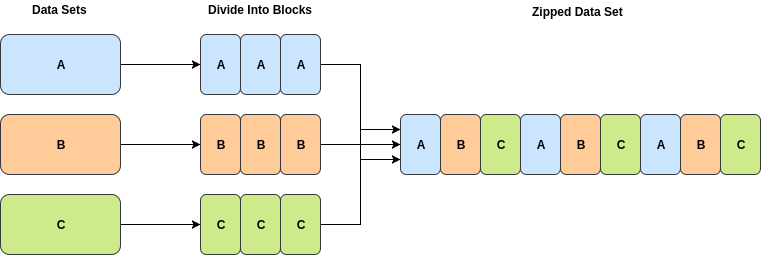
\includegraphics[scale=0.53]{Zip}}
	\caption{Schematic explanation of the zipping procedure to generate train and validation sets.}
	\label{zip}
\end{figure}

\begin{table}[H]
\centering
\begin{tabular}{|c|c|}
\hline
Method & Specification \\
\hline\hline
PCA & 20 principal components \\
Autoencoder & 2 encoding layers, 20 features, Optimization=Adadelta, Loss=MSE\\
Finger Values & Only finger sensors used (41 features) \\
Sum Of Fingers & Sum of sensors for each finger (5 features) \\
Max Of Fingers & Max value for each finger (5 features) \\
\hline
\end{tabular}
\caption{Specifications for the used feature extraction methods.}
\label{FE}
\end{table} 

\begin{table}[H]
	\centering
	\begin{tabular}{|c||c|c|c|c|c|}
		\hline
		 & Box & Sphere & Pyramid & Quarter & Wave \\
		\hline\hline
		Box     & 43.4 (68.2 )& 12.2 (5.2)   & 8.3 (7.8)   & 13.7 (5.8)   & 22.1 (13.2) \\
		Sphere  & 9.0 (6.1)     & 37.0 (62.7)    & 34.7 (11.2) & 12.4 (4.4)   & 6.3 (3.9)\\
		Pyramid & 9.0 (4.7)     & 7.9  (9.0)     & 36.1 (56.0) & 3.3 (4.9)    & 7.4 (6.2)\\
		Quarter & 22.3 (10.1) & 20.6 (11.9)  & 20.8 (14.7) & 64.1 (81.0)  & 6.3 (6.2)\\
		Wave    & 16.3 (10.8) & 22.2 (11.2)  & 0.0 (10.3)    & 6.5 (4.0)    & 57.9 (70.5)\\
		\hline
	\end{tabular}
	\caption{Confusion matrix with values in percent for the target data set and in brackets for the distractor data set.}
	\label{Confusion}
\end{table} 
%----------------------------------------------------------------------------------------
\section{Results and Discussion} \label{results}
\subsection{Classifying Data into Object Categories}\label{e2}
For this experiment the MLP was first trained and evaluated on target data and then on the set containing distractor data. In both cases the training was done individually for each participant and the final score was then calculated by the average over all participants. Both variants were trained multiple times using different feature extraction methods. Each method was evaluated for the tactile data only, the merged set with joint angles concatenated with the tactile data and the joint angles alone.\\ 
The results for the model that was trained on target objects only is shown in Figure \ref{tvt}. Figure \ref{dvd} shows the same experiment but this time trained on the distractor objects. Table \ref{FE} shows the used specifications for the different feature extraction methods. With the PCA the goal was to find a linear transformation for the data whereas the autoencoder with two encoding layers should find a non-linear representation. The other three methods used handcrafted features which were inspired by examining search strategies of participants and finding that most sensory activity can be reduced to the finger sensors. For the joint data no feature extraction method was used. \\
The outcome shows that a training on only the tactile modality yielded best results on both, the target and distractor case. Also noticeable is that when using the merged modalities, a significantly worse performance on the target data can be seen compared to the joint modality while on the distractor set the performance was almost identically between these two. In general, the model performed better on the distractor data which could be due to higher number of data points available.\\
Table \ref{Confusion} shows the confusion matrix for both data sets of this experiment. It appears that the pyramid stimuli has the highest number of confusions relatively for both data sets. Interesting is, that the sphere has the most confusions with the quarter and wave stimuli, which are the only objects besides the sphere that have also rounded features. This brings up the assumption that similar objects are more difficult to separate based on their tactile pattern. 

\begin{figure}
	\centering
	\begin{minipage}{0.496\textwidth}
		\centering
		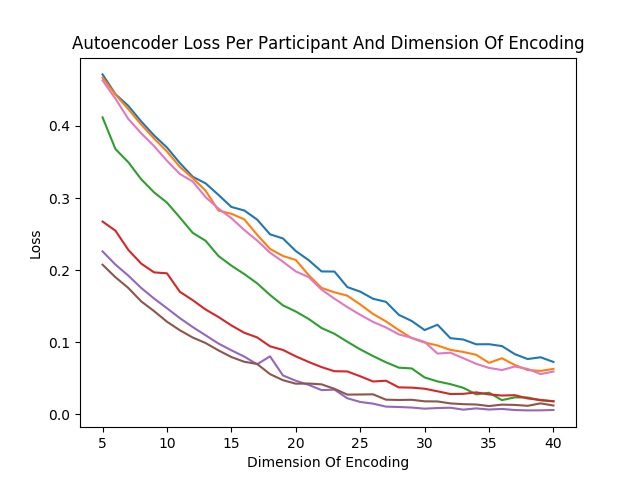
\includegraphics[width=\textwidth]{Autoencoder_loss}
	\end{minipage}
	\begin{minipage}{0.496\textwidth}
		\centering
		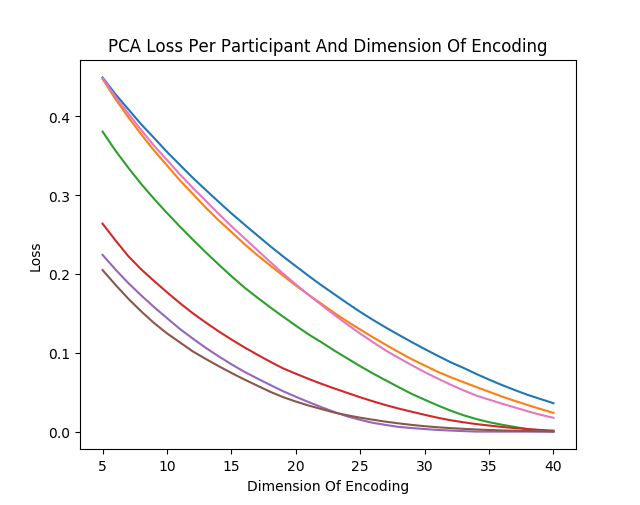
\includegraphics[width=\textwidth]{pca_loss}
	\end{minipage}
	\caption{Reconstruction loss calculated with MSE for each participant. On the left side for the autoencoder and on the right side for the PCA method.}
	\label{ae_pca_loss}
\end{figure}
Even though five different feature methods were tested, none showed considerably better results.\\
An investigation of the reconstruction loss for the autoencoder and PCA method (Figure \ref{ae_pca_loss}) revealed, that not only the performance of the respective model is similar, but also their loss function behavior. It seems that the aspect of linearity or non-linearity in dimensionality reduction does not have significant influence on the reconstruction ability and model performance. Furthermore it can be seen, that there is a high variance for different participants in the loss function.\\
For the following experiments the choice for the feature extraction method fell in favor for taking only the finger sensors, since they showed the most stable results. Also for further investigations the evaluation will be reduced to the tactile modality as there could be seen no improvement for the merged modality or only the joint angles.\\
To evaluate the classifier choice, the chosen modality and features were also tested on other common classifier: a k-nearest-neighbor (KNN) classifier with $ k=10 $ and a support vector machine (SVM) using the radial basis function kernel. Figure \ref{classifier} shows the outcome. For the target data and the tactile modality it can be seen, that the MLP outperforms both other classifiers. Furthermore it shows the least variance amongst the participants. Other modalities tend to have significant higher variance, especially when using only the joint data from the glove. For the distractor case, the MLP on the tactile data outperforms all other results by a large margin. This outcome verifies the decision to take a MLP classifier. 

\begin{figure}
	\centering
	\begin{minipage}{0.495\textwidth}
		\centering
		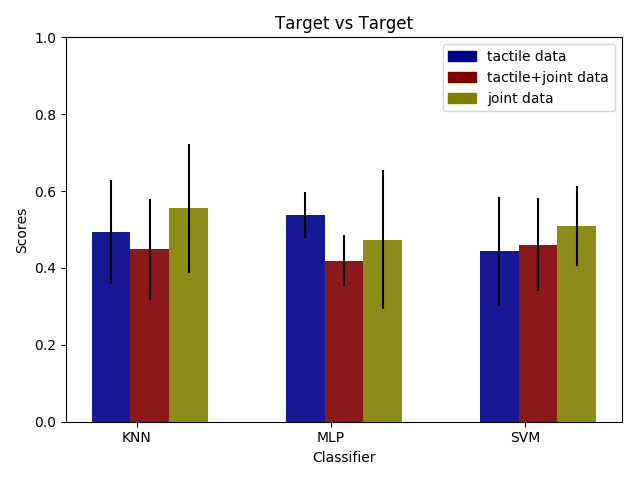
\includegraphics[width=\textwidth]{TvT_c}
	\end{minipage}
	\begin{minipage}{0.495\textwidth}
		\centering
		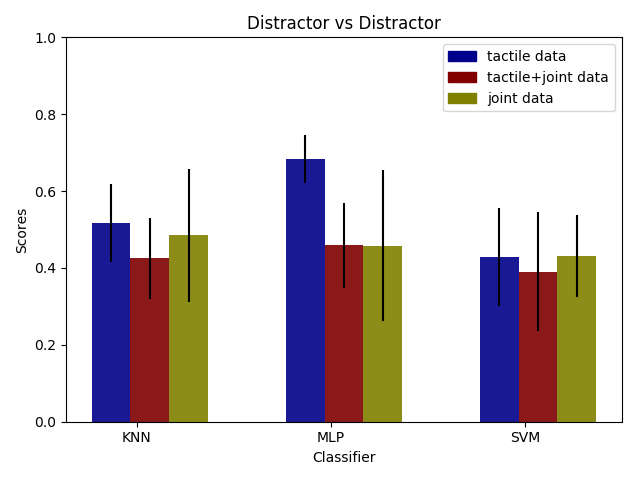
\includegraphics[width=\textwidth]{DvD_c}
	\end{minipage}
	\caption{Scores and variances of KNN, MLP and SVM classifier using three different modalities and the finger sensors as feature vector. On the left side for the target data and on the right side for the distractor data.}
	\label{classifier}
\end{figure}
%For this first problem, four different classifiers were used to test the classification accuracy. In the table below the parameters resulting in the best performance for this task are listed:
%The results for the classifiers that were trained on the target objects only is shown in Figure \ref{tvt}. The score was calculated by averaging the accuracy scores of each participant. The blue bars show the result for the tactile data and the red bars for the merged set that includes joint angles. Also shown is the standard deviation. Figure \ref{dvd} shows the same experiment but this time trained on the distractor objects. For the feature vector 20 principle components yielded the best result as Figure \ref{PCA} shows. It also presents the effect of scaling the data which shows a significant increase of the accuracy.\\
%The results show that for the target data it is possible to classify the five stimuli based on their tactile patterns with an accuracy up to 70\% with the random forest classifier and up to 60\% with the other classifier. Adding the joint angles to the data set however resulted in an small accuracy loss rather than increase.\\
%Comparing these outcomes with the classifier that were trained on the distractor data set, one can see that the performance decreases strongly on latter experiment. Considering a random walk for five classes at 20\%, the models performed just slightly better than it. Interesting is that this time the merged set with joint angles outperformed the solely tactile one in three cases.\\     
%The high variance in both results is based on the participants. The accuracy on some of their data was significantly worse than on other ones. Nonetheless a general trend could be seen for all participants which shows that the random forest classifier performed best in most cases. This model was chosen together with the 20 components for the feature vector for the following experiments.\\ 
%Overall this outcome shows that tactile patterns can be used to classify objects and that the model performs much better on the target data which was assumed. This brings up the hypotheses that rather than as individual objects, humans classify distractors as one class containing mostly object features that does't match the target they searched for. This would at least explain why the classifiers could not really separate the distractor objects. In the following experiments further investigation on this effect will be made. 

\begin{figure}[H]
		\centering
		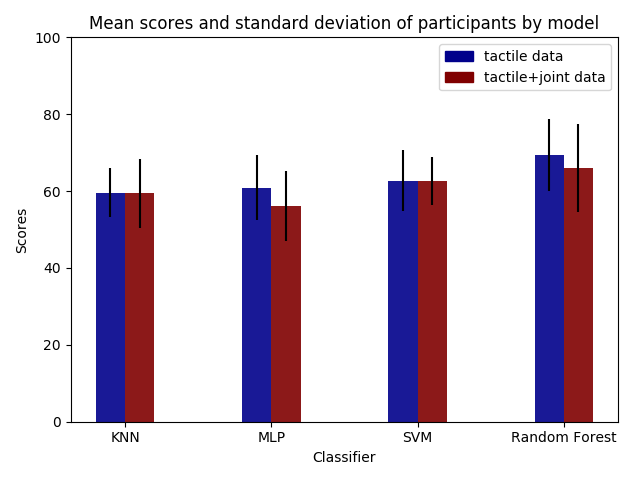
\includegraphics[width=0.9\textwidth]{TvT}
		\caption{Scores of the MLP trained on target data with various feature extraction methods.}
		\label{tvt}
\end{figure}
\begin{figure}[H]
		\centering
		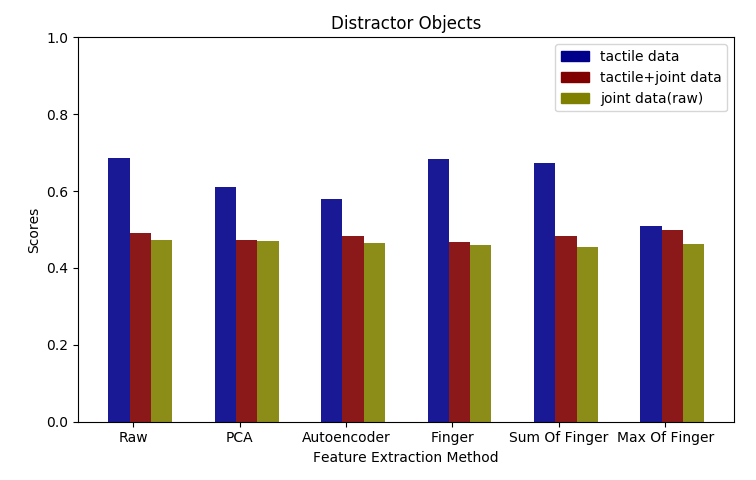
\includegraphics[width=0.9\textwidth]{DvD}
		\caption{Scores of the MLP trained on distractor data with various feature extraction methods.}
		\label{dvd}
\end{figure}


\subsection{Classifying a Single Object as Either Target or Distractor}
This problem is an extension to the previous discussed one. It was found a compelling difference exist in the data regarding the role of an object which can be either target or distractor. For further examinations this problem aimed at finding out whether a classifier can find the role of an object based on the generated tactile data from the exploration. The data was trained with the multilayer perceptron using only finger sensors as features and evaluated with a five-fold cross-validation. \\
Figure \ref{tnt} shows the result of classifying single objects as either target or distractor during the experiment for each stimuli. The accuracy score is composed of the mean scores of the respective objects trained separately on the data for each participant. The outcome shows high scores for all object types on a similar level. Also it can be seen that the pyramid stimuli shows the least accuracy which can be correlated to the confusion matrix (Table \ref{Confusion}) that showed that this object has the least certainty of being correct classified in both, target and distractor data. However, an accuracy of almost 70\% is still achieved. \\
These information proves that the glove can capture the crucial features that determine the objects role in the haptic search and it can be classified with reliable results. In the following experiment it should be further investigated how these roles correlate not only within a single class but on the whole class spectrum.  
 
%Furthermore the outperforming results of the sphere object show additional hints that the assumption from \ref{e2} might be accurate. This stimuli has high differences in its shape compared to the other ones. This means that when this object was a distractor, it was easy for participants to classify it as such. This is reflected by this result since the target and distractor role is well separable in this case as it is for humans. 

\begin{figure}[H]
	\makebox[\textwidth][c]{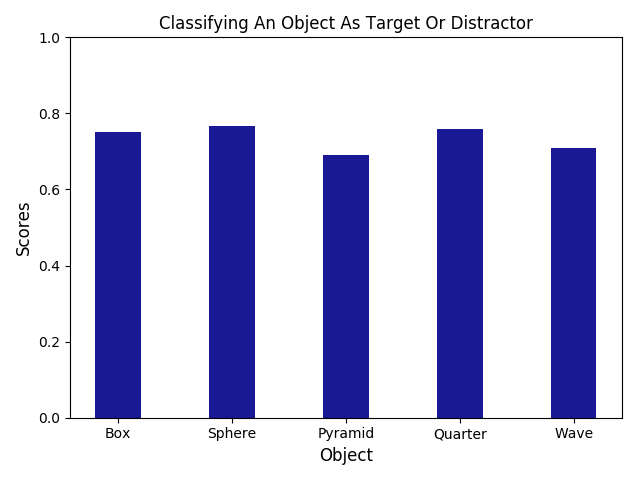
\includegraphics[scale=0.6]{TnT}}
	\caption{Mean scores of MLP trained on data of one object as target and distractor to classify the roles. Only tactile data was used together with the finger sensors as features.}
	\label{tnt}
\end{figure}

\subsection{Classifying unseen Objects into Roles}
%The aim of the last experiment is to find out if all of these assumed features that indicate for a distractor or target object can be separated as just those classes. This would be an additional evidence for the hypotheses that humans classify distractor objects in merely one class rather than the classes of the individual objects themselves as they do for targets. Figure \ref{tvd} shows the results for this experiment. Despite the fact that the distractor objects could not really be separated from each other as \ref{e2} showed, they surely can be discriminated from the target class to at least some degree. The scores of the participants show performance better than random walk, up to 68\%. This outcome reinforces the assumption. Again the merged data set doesn't show significant better scores.
The aim of the last experiment is to find out if it is not only possible to distinguish the roles of one object class, but to see if this will work throughout classes of stimuli objects. For this approach a single object was learned as either target or distractor and tested on a set containing a different unseen object with the same role. Also included in the training and testing was the remaining data with the opposite role of the trained and tested objects. The model should then distinguish between target and distractor data for an unseen object. This will give some insight in the features that are specific for a role and if they are correlated. 

\begin{figure}
	\begin{minipage}[t]{0.49\textwidth}
		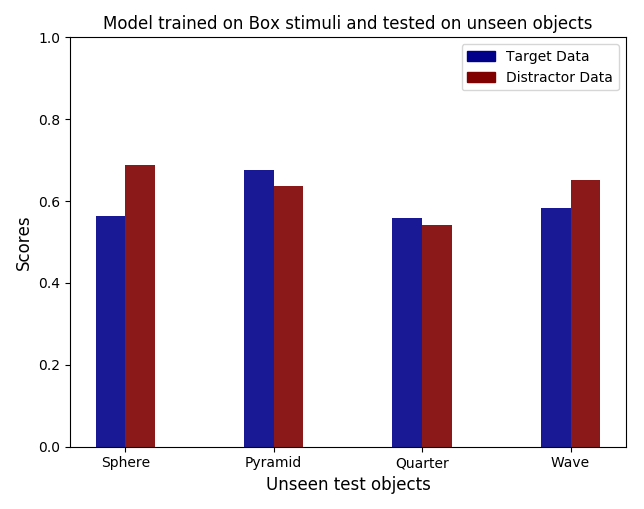
\includegraphics[width=0.965\linewidth]{e3_box}
	\end{minipage}
	\hspace{\fill}
	\begin{minipage}[t]{0.49\textwidth}
		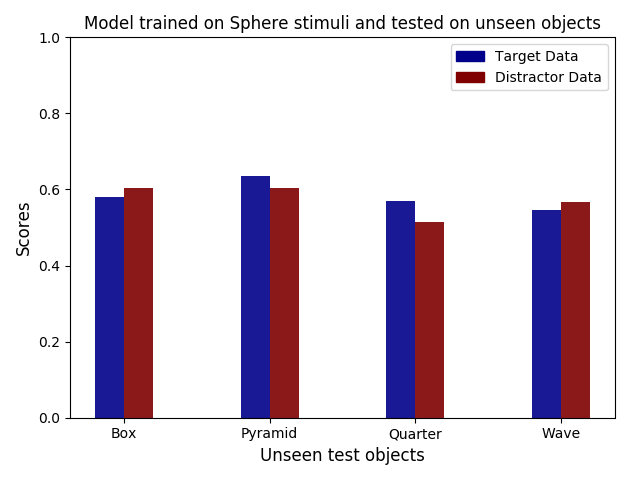
\includegraphics[width=\linewidth]{e3_sphere}
	\end{minipage}
	\caption{On the left side a MLP was trained on the Box stimuli, once as target and distractor and tested on the remaining objects with the respectively roles. The right side shows the same procedure for the Sphere stimuli.}
	\label{e3}
\end{figure}

Figure \ref{e3} shows two cases of this approach. Again, a MLP was trained on solely the tactile modality using the finger sensors as features. The training was done for each subject separately and the scores were averaged. On the left side the Box stimuli was trained once as target and once as distractor and it was tested for one of the remaining stimuli each if it can distinguish between the roles. On the right side the same was done for the Sphere stimuli.\\
The outcome shows that for a model trained only on the Box stimuli, the Pyramid object can be classified with the highest certainty for the target and distractor case. This reinforces the assumption above since this object is the only stimuli besides the Box that has remarkable edges. But still the difference between the objects is small as it is also for the case where the model was trained on the Sphere stimuli. The second case displays even smaller differences. This could be because the Sphere object differs greatly from the other ones which means there are few to none similar features with the other objects.\\
All in all the results don't proof the assumption that there are role specific features since the scores are in a modest range and more testing would be mandatory. However, the scores are better than random which means that the MLP learns some regularity in the data to be able to achieve such scores. 